%% LaTeX2e class for student theses
%% sections/preliminary.tex
%% 
%% Karlsruhe Institute of Technology
%% Institute for Program Structures and Data Organization
%% Chair for Software Design and Quality (SDQ)
%%
%% Dr.-Ing. Erik Burger
%% burger@kit.edu
%%
%% Version 1.1, 2014-11-21
\externaldocument{content}

\chapter{Related Work}
\label{ch:Related Work}
This chapter introduces related and previous works in the realm of Language Identification (LID) and how their approaches differ from the ones employed in the following chapters.

\section{Historically}

As presented in~\cite{zissman1996comparison} by Zissman, Language Identification has historically been the most successful using single-language phone recognition followed by language-dependent, interpolated n-gram language modeling (PRLM) or multiple single-language phone recognizers and language-dependent parallel phone recognition (PPRM). Zissman evaluates PRLM and PPRM as well as the worse performing Gaussian Mixture Models (GMM) on the Oregon Graduate Institute Multi-Language Telephone Speech Corpus (OGI)~\cite{muthusamy1992ogi}. 
In his results on the relatively limited speech corpus of only 90 minutes per language, the PRR perform the best with an 2-Language Average Error of 8 \% and the GMM falling down to an error of 23 \%.

In ~\cite{torres2002approaches}, Torres-Carrasqiullo et al. present two GMM-based approaches to LID that use shifted-delta- cepstral (SDC) coefficients as the feature input vectors to achieve comparable LID (and computationally much faster) results. In opposition to PRLM and PPRM, GMM use the acoustic content of the speech signal to classify languages. The GMM with SDC inputs fare the same as PPRM on the CallFriend Corpus~\cite{callfriend1996}. The same OGI test set as~\cite{zissman1996comparison} for 10-second utterances, is only about 9 \% worse for GMM. However they start being greatly outperformed by PPRM in longer 45 second utterances. GMM do have a significant lesser computational overhead~\cite{zissman1996comparison}~\cite{torres2002approaches}, and do not require \textit{a priori} information (phonetic transcriptions) to be available~\cite{zissman2001automatic},~\cite{zissman1996comparison} making their research still worthwhile, however.

\section{Recent Approaches}
Li et al. in \cite{4032773}, used vector space modeling (VSM) in combination with the already presented PPRM to calculate the distance between different languages more easily thus making classification easier. By determining the top most occurring words in a language, they rely on these statistics to distance languages from each other, then applying a language-dependent language model on top to classify. A similar approach is proven to be successful with support vector machines (SVM) in~\cite{4590023},~\cite{6289007} and further substantiated in~\cite{ma2006comparative} where the SVM approach performs the best out of a comparison with the older PPRM and VSM methods.
\par
Recently with the advance of Neural Networks in Machine Learning, many different approaches have been tried. Leena et al. in~\cite{1529486} present a Feed-Forward Neural Network that is trained using both phonotactic (syllable occurrence, co-occurrence of syllables, unique syllables and pronunciation variations) and prosodic (rhythm and intonation of speech) features, giving a feature vector of 33 dimensions, to recognize the Language. Leena et al also use autoassociative neural networks and spectral similarity approaches in~\cite{1287674} to recognize language reasonably well using only a few seconds of the speech as input.

\par

I-vector approaches as in~\cite{6680440},~\cite{d2012phonotactic} have also recently shown success, and have been used in conjunction with neural networks as in~\cite{song2015deep}.

\section{Similar Approaches}
Matejka et al.~\cite{matejka2014neural} present an approach very similar to the one introduced in this thesis using Bottleneck Features (BNF) from an ASR trained neural network as input for a LID neural network. Here however a much bigger train data of about 400 hours per language is available in the RATS LID Data Corpus, than was available to us, with fewer target languages and a setup where the output of 5 neural networks is averaged, a setup most likely occurring a higher delay than feasible in an online-setting as the focus lies on for us.

\cite{6854622} uses Deep Neural Networks without the previous ASR net setup to identify Language. They compare the approach to state-of-the art i-vector as presented above.



This work is based on previous work done using LID information to extract another BNF vector to then aid in multilingual ASR~\cite{Mueller2016b}. More on this can be found in Chapter~\ref{ch:LITasks}.

\chapter{Fundamentals}
\label{ch:fund}

The following chapter will define and explain terms and concepts used throughout this thesis, as to make understanding of the following chapters easier.

\section{Theory of Language Identification}

Language Identification, or Recognition, as loosely taken from~\cite{6451097}, can be formulated in the following way: Assuming we have an audio recording of unknown source language, we convert it into a sequence of acoustic vectors \(S = \{ s(1), s(2), \dots , s(T)\}\), where \(s(t)\) refers to frame extracted from the audio at frame number \(t\). If we have a set of possible equally-probable Languages \(\{L_1,L_2,\dots,L_N\}\), with one of the targets being a combining class for non-target languages as to not limit the approach, Language Identification is the task of finding optimal Language \(L^O\) given audio sequence \(S\) , such that:
\begin{equation}
L^O = \argmax_I p(S|L_I)
\end{equation}
Using phones and phonotactic knowledge sources, or a tokenizer or similar approaches before trying to identify the language, we assume that each speech sequence can be segmented into a sequence \(\Upsilon\) of phones \(\upsilon\) which means:
\begin{equation}
\label{eq:phones}
L^O = \argmax_I P(\Upsilon|L_I)
\end{equation}

While in \ref{eq:phones} we assume to know the exact phoneme sequence, in practice \(\Upsilon\) has to be retrieved by selecting the most likely phone sequence from all possible sequence. Using Viterbi Decoding on a set of phone models \(M\) we can retrieve the optimal \(\Upsilon^O\):
\begin{equation}
\label{eq:phonesO}
\Upsilon^O = \argmax_{\upsilon} P(S|\upsilon, M)
\end{equation} 

Combining \ref{eq:phones} and \ref{eq:phonesO} and considering all possible \(\Upsilon\) instead of the best hypothesis \(\Upsilon^O\) we get:
\begin{equation}
L^O = \argmax_{I}\sum_{\forall \Upsilon}P(S|\Upsilon, M)P(\Upsilon|L_I)
\end{equation}

\section{Janus Recognition Toolkit (jrtk)}
\label{sec:fund:jrtk}
The Janus Recognition Toolkit (jrtk) also known as just ``Janus'' is a general-purpose speech recognition toolkit developed in joint cooperation by both the Carnegie Mellon University Interactive Systems Lab and the Karlsruhe Institute of Technology Interactive Systems Lab~\cite{lavie1997janus}. Part of janus and the jrtk are a speech-to-speech translation system which includes Janus-SR the speech recognition component, the main part of janus used in this thesis. 

Developed to be flexible and extensible, the jrtk can be seen as a programmable shell with janus functionality being accessible through objects in the tcl/tk scripting language. It features the IBIS decoder, that uses Hidden Markov Models for acoustic modeling in general, although in this thesis we used a neural network as our speech recognizer to generate the input features required by our Language ID network.

This thesis makes extensive use of the jrtk's and tcl/tk's scripting capabilities to be able to pre-process speech audio files for further use by our experimental setup. It also uses tcl/tk scripts and it's janus API functionality in the development of our smoothing and evaluation scripts as can be seen in Ch.~\ref{ch:eval}.
\section{Neural Networks}
\label{sec:fund:NN}
Artificial Neural Networks today are used in many different fields: from image recognition/face recognition in~\cite{lawrence1997face} to Natural Language Processing in~\cite{collobert2008unified} and, as relevant to this thesis, to Speech Recognition and very successfully as in~\cite{hinton2012deep}. It has also been used in the realm of Language Identification, which has been described in the previous chapter. This section will provide fundamental knowledge of how neural networks work and how to train them, to make the understanding of later chapters easier for the reader. The information in this section is based on~\cite{haykin2004comprehensive}, ~\cite{Goodfellow-et-al-2016} and~\cite{deeplearning-online}, if not otherwise sourced.


\subsection{Neural Networks}
\label{sec:fund:general}
Neural Networks are based on collections of small ''neural units``  working together in tandem. The neuron's behavior can be loosely linked to the brain's axons. Each neuron is connected with others and a neuron is ''stimulated`` by input on these connections and then decides on its own activation, or stimulation, by using a summation, or threshold, function with a certain limit to decide if the neuron ''fires`` and its own activation is propagated through the network to adjacent units. By changing weigths and activation thresholds in the network its output changes, therefore the possible adjustable parameter set \(\Theta\) for a neural network includes all the weights for all neurons as well as all thresholds for the activation functions in each neuron.

\subsection{Artificial Neuron}
\label{sec:fund:AN}

An artificial neuron, or perceptron in its most basic form, is a mathematical function that consists of four parameters that can be adjusted independently from each other:
\begin{itemize}
\item \(w_i\) the input weights for all inputs
\item \(\Sigma\) the transfer function for summation of the weighted inputs
\item \(\varphi\) the activation function that calculates the output value \(y_k\) basend on the transfer input and the threshold
\item \(\theta\) the threshold which defines when the neuron activates.
\end{itemize}

This means an artificial neuron with output \(y_k\) is the function~\ref{eq:an}. Many of these neurons coupled together (via the output of a neuron on a previous layer becoming the input for one on the current layer), make an Artificial Neural Network as used in this thesis. A schematic drawing of this can be seen in Fig.~\ref{fig:neuron}.

\begin{equation}
y_k = \varphi(\sum_{j=0}^{m} w_{kj}x_j) - \theta_j
\label{eq:an}
\end{equation}

\begin{figure}[h!]
\label{fig:neuron}
\caption{A schematic drawing of a Neuron and it's parameters}
\centering
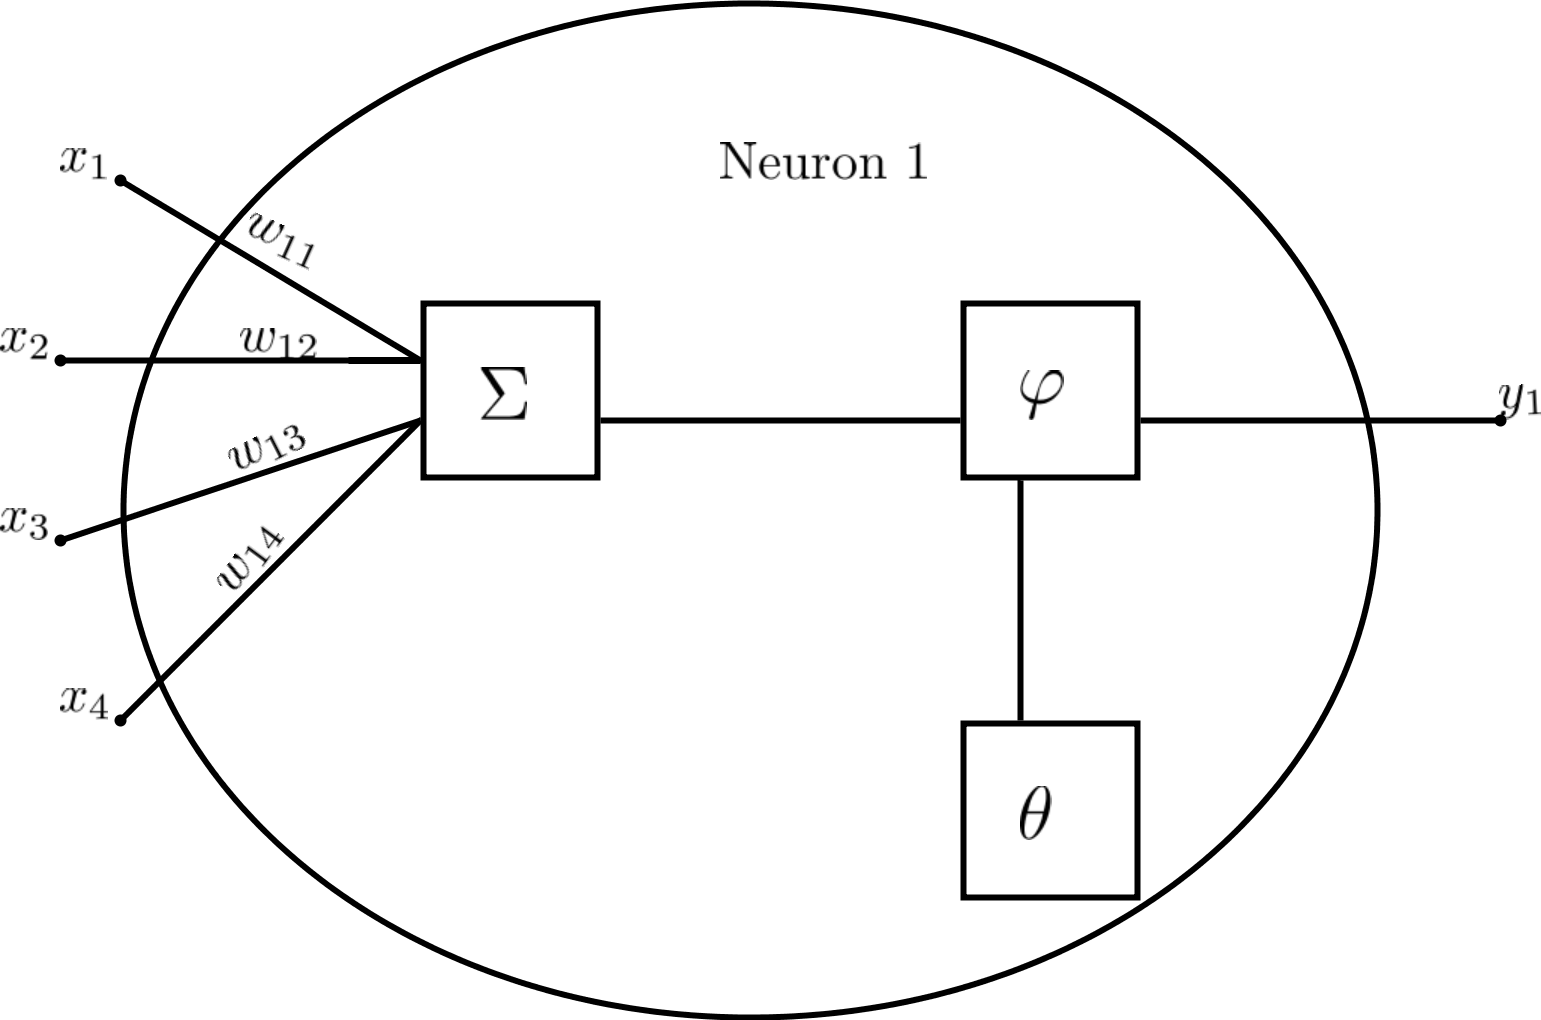
\includegraphics[width=0.7\textwidth]{images/neuron.png}
\end{figure}

\subsection{General Network Setup}
\label{sec:fund:netSetup}

A basic neural network consists of three layers: the input, a hidden layer of neurons and the output layer. Hereby, the output layer consists of as many neurons as classes that the network is trying to classify against and the one with the highest activation after entering input, is the classification output of the net.  A basic, fully-connected (referring to the connections between neurons, so fully-connected means each neuron is connected to each possible other neuron) net can be seen in Fig.~\ref{fig:net}.
\tikzstyle{layer}=[draw=black,fill=black!30]
\tikzstyle{layerlid}=[draw=black,fill=green!30]
\tikzstyle{dots}=[draw=black,fill=black]
\begin{figure*}[htbp]
   \centering

   \begin{tikzpicture}[scale=1.0]

   % Input Layer

   \draw (-1.75, 2.5) node[draw=white,fill=white] {Input Features};

   \fill[layer] (-2,0.5) coordinate(l0bl) -- (-1.5,0.5) coordinate(l0br) --
(-1.5,1.5) coordinate(l0tr) -- (-2,1.5) coordinate(l0tl) -- (-2,0.5);

   \fill[layer] (-2,-0.5) coordinate(l0_1bl) -- (-1.5,-0.5) coordinate(l0_1br)
-- (-1.5,0.5) coordinate(l0_1tr) -- (-2,0.5) coordinate(l0_1tl) -- (-2,-0.5);

   \draw[dots] (-1.75,-0.7) circle (0.045);
   \draw[dots] (-1.75,-0.875) circle (0.045);
   \draw[dots] (-1.75,-1.05) circle (0.045);

   \fill[layer] (-2,-2.25) coordinate(l0_2bl) -- (-1.5,-2.25)
coordinate(l0_2br) -- (-1.5,-1.25) coordinate(l0_2tr) -- (-2,-1.25)
coordinate(l0_2tl) -- (-2,-2.25);

   % Output Stack
   \fill[layer] (4,0.5) coordinate(l5bl) -- (4.5,0.5) coordinate(l5br)
-- (4.5,1.5) coordinate(l5tr) -- (4,1.5) coordinate(l5tl) -- (4,0.5);
   \fill[layer] (4,-0.5) coordinate(l5_1bl) -- (4.5,-0.5)
coordinate(l5_1br) -- (4.5,0.5) coordinate(l5_1tr) -- (4,0.5)
coordinate(l5_1tl) -- (4,-0.5);

   \draw[dots] (4.25,-0.7) circle (0.045);
   \draw[dots] (4.25,-0.875) circle (0.045);
   \draw[dots] (4.25,-1.05) circle (0.045);

   \fill[layer] (4,-2.25) coordinate(l5_2bl) -- (4.5,-2.25)
coordinate(l5_2br) -- (4.5,-1.25) coordinate(l5_2tr) -- (4,-1.25)
coordinate(l5_2tl) -- (4,-2.25);

   \draw (1.5,-2.7) node {Hidden Layer};

   \draw (4.25,2.5) node[draw=white,fill=white] {Output Classes};

   % Hidden layer

   \fill[layer] (1.0,-2.25) coordinate(l4bl) -- (1.5,-2.25) coordinate(l4br)
-- (1.5,1.5) coordinate(l4tr) -- (1.0,1.5) coordinate(l4tl) -- (1,-2.25);


  
   \draw (l0tr) -- (l4bl);
   \draw (l0_2br) -- (l4tl);
   \draw (l4tr) -- (l5_2bl);
   \draw (l4br) -- (l5tl);

   \end{tikzpicture}
   \caption{Basic Feed-Forward fully-connected Neural Network.}
   \label{fig:net}
\end{figure*}
\subsection{Network Types}
\label{sec:fund:types}

\subsubsection{Feed-Forward Neural Networks}
A basic (non-deep) \textit{Feed-Forward Neural Network} consists of three layers: the input, a hidden layer of neurons and the output layer. Feed-Forward refers to the fact, in opposition to \textit{Recurrent Neural Networks}, that connections between the neural units are not cyclic. 

In such a basic network, the output layer consists of as many neurons as classes that the network is trying to classify against and the neuron with the highest activation after entering input, is the classification output of the net.

\subsubsection{Deep Feed-Forward Neural Networks}
\textit{Deep Feed-Forward Neural Networks}, DNNs, the net-type most used in this thesis, refer to Networks that have more than one hidden layer between input and output, but still feature non-cyclic connections between neurons. DNNs have a better performance than single-hidden-layer-networks in general, but require different techniques for training. 

A common description of this phenomen is, that each hidden layer increases the level of abstraction the network can manage. E.g, in image processing, if the first layer recognizes a color in a certain pixel, then the next layer can infer more abstract characteristics from the output of the first layer. For example, after knowing a certain pixel is dark the next layer can derive that area might be the eye in a picture of a face, etc. This obviously makes more complicated classification tasks possible but also makes learning algorithms more difficult.

\subsubsection{Deep Recurrent Neural Networks}
\textit{Deep Recurrent Neural Networks}, RNNs, refer to neural networks that are DNN's but cyclic connections are allowed. This means the network can have temporal behavior, so its performance changes dynamically over time, when the state of later neurons changes and affects the neurons in previous layers.

\paragraph{Long-Short-Term-Memory} The most common RNNs are based on Long-Short-Term-Memory units, artificial neurons that can remember values for a short or long duration, thus having an internal state that changes over time and does not have an activation function like normal artificial neurons. Normally, RNNs then include LSTM blocks of multiple LSTM units. The LSTM blocks then control the change of memory through ``gates''. The input gate to control when a new value is entered into memory, the forget gate to control if a value remains in memory and the output gate which controls the calculation of the activation of the entire block. The weights that are learned for LSTM blocks are then used in front of the gates. That means the weight determines the values of the memory in the block and therefore the activation. RNNs are trained with a similar algorithm as introduced in the next section for non-recurrrent networks, called Backpropagation through time. A detailled explanation of this can be found in~\cite{58337}.


\subsection{Learning}
\label{sec:fund:Learn}
The interesting part about Neural Networks is their ability to learn from data and improve their own performance. Improving performance in this case means that by adjusting the available parameters of the neurons part of the network, we minimize a cost function that describes the difference between an optimal output and the actual output. 

A Network can be seen to be an approximation of a function \(f^*\). So, a network trying to classify an input \(x\) into a class \(y\) approximates:
\begin{equation}
\label{eq:learn}
y=f^*(x)
\end{equation}
Then one run of the Network with parameter set \(\Theta\) gives the mapping \(y = f(x;\Theta)\) and we are trying to minimize our cost function of \(C= f^* - f\) by adjusting the set of parameters in \(\Theta\) each run.

\paragraph{Three basic approaches exist for training a network:} \hspace{0pt} \\
\begin{itemize}
\item \textit{Supervised Training}, where the optimal output for input train data is known. This means, the train data has been pre-classified by a ``teacher''. This is the method we use in this thesis and further explained below.
\item \textit{Reinforcement Training}, where the optimal input for train data is not known prior to training, but the environment gives the net feedback about its own output and good output is ``reinforced'' while bad output is discouraged.
\item \textit{Unsupervised Training}, where nothing is known about the environment and the net (often) just tries to learn the probabilistic distribution of the data.
\end{itemize}

\subsubsection{Sampling}
\label{sec:fund:Sampling}

Data for training is generally split into three sets: the training set with a size of about \(80\%\) of the total available data which is then used for the training, the development set with a size of about \(10\%\) used for evaluation of the net and adjusting different parameters without ``distorting'' the last test set which also has a size of around \(10\%\) and is used for final ``clean'' validation of the net performance.


Sampling for the three sets is most commonly, as in this thesis, done using Simple Random Sampling (SRS), where each set is chosen randomly and completely by chance so that each sample has the same chance to be part of any of the three sets, and furthermore any combination of \(n\) samples has the same probablity to be in any of the sets~\cite{meng2013scalable}

\subsubsection{Supervised Training}
\label{sec:fund:ST}
Supervised Training refers to training where the optimal output for the training data is known, so a classification of the train data exists prior to training. This makes calculation of the Cost function as defined in the previous section relatively easy, as we define \(C\) as the actual difference in output of the current net with current parameter set \(\Theta\) compared to the teacher-defined classification/labeling. 

\paragraph{Mean Squared Error Function}

One way to calculate the difference between the net and the teacher-classification is by using the mean squared error, as is used in the training of nets in this thesis. If  \(t\) is the expected output and \(f(x;\Theta)\) is the actual predicted output and \(M\) the number of output neurons/classes, we define the Mean Squared Error (MSE) as:
\begin{equation}
E = 1 / 2 \sum_{j=1}^{M}(f(x;\Theta) - t)^2
\end{equation}

\paragraph{Stochastic Gradient Descent} The goal of course is to minimize the MSE as defined above by adjusting parameters for each neuron and layer (including weights to output neurons) to change the predicted output of the net.  This is done by adjusting the weights in direction of the falling gradient for each weight.
\begin{equation}
w_{i+1} = w_i - \eta \nabla E(f(x;w), t) = w_i - \eta \nabla 1/2\sum_{j=1}^M(f(x;w) - t)^2
\end {equation}

This method is called the ``Gradient Descent'', with \(\eta\) being the ``Learning Rate'', the freely adjustable speed at which the network changes and therefore learns. As calculation of this gradient for every sample in the training data set is expensive, a stochastic approach is used where only a small number of samples is used each iteration to calculate the gradient, as the relation between the change of the mean error and the value of samples is not linear. Therefore the calculation of the ´´Stochastic Gradient Descent'' (SGD) is enough to estimate the real required parameter-changes.

\paragraph{Backpropagation} While the SGD is used to calculate each iterative weight according to the falling gradient, the Backpropagation algorithm is used to calculate each weight from the total output of the net and its input. If we have neural network output vector (all output neurons together) \(t_i\), input vector (all input dimensions together) \(x_i\) and current weights \(w_i\) we can calculate \(w_{i+1}\) by calculating the SGD on the function \(w \rightarrow E(w, x_i), y_i)\).

With preceding definitions we can summarize the training algorithm of a DNN as follows:
\definecolor{green}{rgb}{0.0, 0.4, 0.13}
\lstset{captionpos=b,tabsize=3,frame=lines,keywordstyle=\color{blue},commentstyle=\color{green},stringstyle=\color{red},numbers=left,numberstyle=\tiny,numbersep=5pt,breaklines=true,showstringspaces=false,basicstyle=\footnotesize,emph={label}}
\begin{lstlisting}[label=lst:pseudo:train,caption=Pseudo Code to show the Backpropagation/SGD algorithm in Action,mathescape]
 $\displaystyle w_0 := rand()$
  do
     forEach train-sample s
        $\displaystyle f(x;w_i)$ = neural-net-output$\displaystyle(w_i, s) $ // Actual calculation using each neurons output -> Forward pass
        t = pre-classification(s)
        Error = $\displaystyle E(f(x;w_i), t)$
         $ \displaystyle w_{i+1}:=  w_i - \eta \nabla E(f(x;w), t) = w_i - \eta \nabla 1/2\sum_{j=1}^M(f(x;w) - t)^2$  //For all Weights and layers -> Backwards pass
        $\displaystyle w :=w_{i+1}$
   if ($\Delta E$ <= Threshold) break
return Net
\end{lstlisting}
